%%%%%%%%%%%%%%%%%%%%%%%%%%%%%%%%%%%%%%%%%%%%%%%%%%%%%%%%%%%%%%%%%%%
% 
% $Id: secn.tex,v 1.1.1.1 2002/01/02 19:36:28 phil Exp $
%
% $Log: secn.tex,v $
% Revision 1.1.1.1  2002/01/02 19:36:28  phil
% initial import into CVS
%
% Revision 1.1  2001/12/16 07:17:39  phil
% Initial revision
%
% Revision 1.11  1997/08/29 20:06:09  allen
% *** empty log message ***
%
% Revision 1.10  1997/08/28 16:38:31  cguo
% *** empty log message ***
%
% Revision 1.9  1996/08/13 19:10:50  phil
% uncommented \technicalnote
%
% Revision 1.8  1996/08/13 17:10:52  cguo
% *** empty log message ***
%
% Revision 1.7  1996/08/13 00:56:11  cguo
% glossary a problem
%
% Revision 1.6  1996/08/12 23:19:35  phil
% ready for carmen to finish \emph
%
% Revision 1.5  1996/08/12 21:27:45  cguo
% test problem with quote
%
% Revision 1.4  1996/08/02 22:17:59  cguo
% *** empty log message ***
%
% Revision 1.3  1996/04/29 19:02:55  stockie
% ready for carmen
%
% Revision 1.2  1995/08/14  22:16:15  stockie
% - add glossary definitions
% - change labels to depend on lab #
% - remove color commands
% - update quiz, technicalnote, and other environments
% - add comments for figures
% - add technicalnote's
%
% Revision 1.1  1995/07/18  21:38:41  stockie
% Initial revision
%
%
%%%%%%%%%%%%%%%%%%%%%%%%%%%%%%%%%%%%%%%%%%%%%%%%%%%%%%%%%%%%%%%%%%%

\section{Introduction: Why bother with numerical methods?}
\label{lab1:sec:intro}

In introductory courses in ordinary and partial 
differential equations (ODE's and PDE's), 
many analytical techniques are introduced for deriving solutions.
These include the methods of undetermined coefficients, variation
of parameters, power series, Laplace transforms, separation of
variables,  Fourier series, and phase plane analysis, to name a few. 
When there are so many analytical tools available, one is led to ask:

\begin{quote}
\centerline{\emph{Why bother with numerical methods at all?}}
\end{quote}

The fact is that the class of problems that can be solved
analytically is \emph{very small}.  
Most differential equations that 
model physical processes cannot be solved explicitly, and the only
recourse available is to use a numerical procedure to obtain
an approximate solution of the problem.  

%%%%%
\begin{latexonly}
\gloss{ordinary differential equation}{a differential
  equation where the derivatives appear only with respect to one
  independent variable.  Abbreviated ODE.} 
\gloss{independent variable}{a variable that does not depend
  on other quantities (typical examples are time, position, etc.)}
\gloss{dependent variable}{a variable which is
  a (possibly unknown) function of the independent variables in a
  problem; for example, in a fluid the pressure can be thought of as a
  dependent variable, which depends on the time $t$ and position
  $(x,y,z)$.}   
\gloss{ODE}{see \emph{ordinary differential equation}}
\gloss{partial differential equation}{a differential
  equation where derivatives appear with respect to more than one
  independent variable.  Abbreviated PDE.} 
\gloss{PDE}{see \emph{partial differential equation}}
\gloss{differential equation}{an equation involving derivatives.
  Abbreviated DE.} 
\gloss{DE}{see \emph{differential equation}}
\gloss{linear interpolation}{interpolation using straight lines between 
the known points}
\end{latexonly}
%%%%%

Furthermore, even if the
equation can be integrated to obtain a closed form expression for the
solution, it may sometimes be much  
easier 
to approximate the solution numerically than to evaluate it
analytically.

In the following two sections, we introduce two classical physical
models, seen in most courses in differential equations.  Analytical
solutions are given for these models, but then seemingly minor
modifications are made which 
%% render the problem mathematically intractable, 
make it difficult (if not impossible) to calculate actual solution
values using analytical techniques.  
The obvious alternative is to use numerical methods.

%%%%%%%%%%%%%%%%%%%%%%%%%%%%%%%%%%%%%%%%%%%%%%%%%%%%%%%%%%%%%%%%%%%%%%%
\subsection{Ordinary Differential Equations}
\label{lab1:sec:odes}

In order to demonstrate the usefulness of numerical methods, let's
start by looking at an example of a \emph{first-order initial value
  problem} (or \emph{IVP}).  
In their most general form, these equations look like
\begin{equation}
  \begin{array}{c}
    {\displaystyle \frac{dy}{dt} = f(y,t),} \\
    \; \\
    y(0) = y_0, 
  \end{array}
  \label{lab1:eq:modelode} 
\end{equation}
where
\begin{itemize}
\item $t$ is the \emph{independent variable} (in many physical systems,
  which change in time, $t$ represents time);
\item $y(t)$ is the unknown quantity (or \emph{dependent variable}) that
  we want to solve for;
\item $f(y,t)$ is a known function that can depend on both $y$ and
  $t$; and 
\item $y_0$ is called the \emph{initial value} or \emph{initial
    condition}, since it provides a value for the solution at an
  initial time, $t=0$ (the initial value is required so that the
  problem has a unique solution).
\end{itemize}
This problem involves the first derivative of the solution, and
also provides an 
initial value for $y$, and hence the name ``first-order initial value
problem''.   

Under certain very general conditions on the right hand side function
$f$, we know that there will be a unique solution to the problem
\eqref{lab1:eq:modelode}.  However, only in very special cases can we
actually write down a closed-form expression for the solution.
 
In the remainder of this section, we will leave the general equation,
and investigate a specific example related to heat conduction.
It will become clear that it is the problems which \emph{do not have
  exact solutions} which are the most interesting or meaningful from a
physical standpoint.  

\begin{latexonly}
\gloss{initial value problem}{a differential equation (or set
of differential equations) along with
  initial values for the unknown functions.  Abbreviated IVP.}
\gloss{IVP}{initial value problem}
\gloss{boundary value problem}{a differential equation (or set
of differential equations) along with
  boundary values for the unknown functions.  Abbreviated BVP.}
\gloss{BVP}{see \emph{boundary value problem}}
\gloss{first order differential equation}{a differential equation
  involving only first derivatives of the unknown functions.}
\gloss{second order differential equation}{a differential equation
  involving only first and second derivatives of the unknown
  functions.}
\end{latexonly}

\begin{example}
  \label{lab1:exm:conduction}
  Consider a small rock, surrounded by air or water, which gains or
  loses heat only by conduction with its surroundings 
  (\ie there are no radiation effects).
  If the rock is small enough, then we can ignore the effects of
  diffusion of heat within the rock, and consider only the flow of heat
  through its surface, where the rock interacts with the surrounding
  medium.  

  It is well known from experimental observations that the 
  rate at which the temperature of the rock changes
  is proportional to 
  the difference between the rock's surface temperature, $T(t)$, 
    and the \emph{ambient temperature}, $T_a$
  (the ambient temperature is
  simply the temperature of the surrounding material, be it air,
  water, \dots).
  This relationship is expressed by the following ordinary
  differential equation
  \begin{equation}
%    \textcolor[named]{Red}{\frac{dT}{dt}} = -\lambda \,
%    \textcolor[named]{Blue}{(T-T_a)} .
    \underbrace{\frac{dT}{dt}}_{\begin{array}{c} 
                                \mbox{\rm rate of change}\\
                                \mbox{\rm of temperature}
                                \end{array}}
    = -\lambda \underbrace{(T-T_a)}_{\begin{array}{c} 
                                \mbox{\rm temperature}\\
                                \mbox{\rm difference}
                                \end{array}} .
    \label{lab1:eq:conduction1d}
  \end{equation}
  and is commonly known as \emph{Newton's Law of Cooling}.
  (The parameter $\lambda$ is defined to be $\lambda = \mu A/cM$, where
  $A$ is the surface area of the rock, 
  $M$ is its mass, $\mu$ its thermal conductivity, and $c$ its
  specific heat.)

  \quiz{quiz-conduction.html}{Here is a short quiz on Newton's Law of Cooling.} 
  
  If we assume that $\lambda$ is a constant, then the solution to this
  equation is given by 
  \begin{equation}
    T(t) = T_a + (T(0)-T_a)e^{-\lambda t},
    \label{lab1:eq:conduction-soln}
  \end{equation}
  where $T(0)$ is the initial temperature.  
  
  \begin{mathnote} 
    \hyperref{Details of the derivation \dots}{See Appendix }{ for a
      derivation of the solution.}{lab1:ap:conduction}
  \end{mathnote}
  
  In order to obtain realistic value of the parameter $\lambda$,
  let our ``small'' rock be composed of granite, with mass of
  $1\;gram$, which corresponds to a   
  $\lambda \approx 10^{-5}\;sec^{-1}$.  
%  We then have approximate values of 
%    $M = 10^{-3}\;kg$, 
%    $A = 10^{-5}\;m^2$, which gives
% THIS MU IS WRONG!  IT'S DIMENSION OF metres^{-1} DOESN'T MAKE SENSE!
%    $\mu = 3.5 \times 10^{-3}\;J(m\,sec\,^{\circ}C)^{-1}$,
%    $c = 8.0 \times 10^{2}\;J(kg\,^{\circ}C)^{-1}$, and
%    $\lambda \approx 0.44 \times 10^{-7} sec^{-1}$.

%
% This figure generated by the Gnuplot script 
% conduction/conduction.gin
% 
\begin{latexonly}
    Sample solution curves are given in Figure~\ref{lab1:fig:conduction}.
    \begin{figure}[htbp]
      \begin{center}
        \leavevmode
%%%%%%%%%%%%%%%%%%%%%%%%%%%%%%%%%%%%%%%%%%%%%%%%%%%%%
%  NOTE: This plot is produced by the Gnuplot script
%  ``conduction/conduction.gin''.  
%%%%%%%%%%%%%%%%%%%%%%%%%%%%%%%%%%%%%%%%%%%%%%%%%%%%%
%        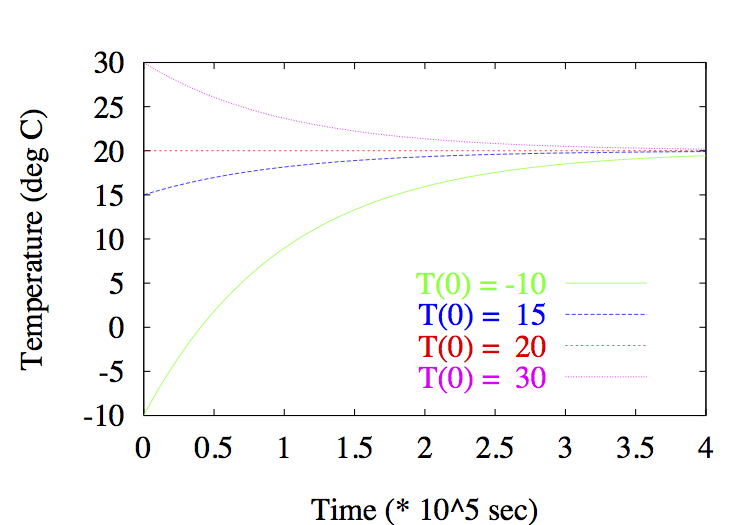
\includegraphics[height=3.5in]{conduction/conduction.pdf}
        \caption{Plot of solution curves $T(t)$ for $T_0=-10,15,20,30$;
          parameter values: $\lambda=10^{-5}$, $T_a=20$.} 
        \label{lab1:fig:conduction}
      \end{center}
    \end{figure}
\end{latexonly}

\demo{conduction.cgi}{Here is an interactive example that investigates
  the behaviour of the solution.\label{lab1:demo:conduction}}

\technicalnote{Details on how the conduction example works\dots}{See Appendix }{ for details on how the conduction example works.}{lab1:tech:conduction}  

\end{example}

\begin{example}
  \label{lab1:exm:conduction-nonlinear}
  Suppose that the rock in the previous example has a $\lambda$
  which is \emph{not} constant.  For example, if
  that the rock is made of a material whose specific heat varies with
  the temperature or time, then $\lambda$ can be a function of $T$ or
  $t$.  
  This might happen if the material composing the
  rock undergoes a phase transition at a certain critical temperature
  (for example, a melting ice pellet).  
  The problem is now a \emph{non-linear} one, for which analytical
  techniques may or may not provide a solution.

  If $\lambda=\lambda(T)$, a function of temperature only, then the
  exact solution may be written as 
  \[ 
  T(t) = T_a + \exp{\left[-\int^{t}_{0} \lambda(T(s))ds \right]},
  \]
  which involves an integral that may or may not be evaluated
  analytically, in which case we can only approximate the integral.  
  Furthermore, if $\lambda$ is a function of both $T$ and $t$ which is
  \emph{not separable} (\ie cannot be written as a product of a
  function of $T$ and $t$), then we may not be able to write down a
  closed form for the solution at all, and we must resort to
  numerical methods to obtain a solution.

  Even worse, suppose that we don't know $\lambda$ explicitly as a
  function of temperature, but rather only from experimental
  measurements of the rock (see Figure~\ref{lab1:fig:table} for an
  example).   
  Then there is no way to express the rock's temperature as a
  function, and analytical methods fail us, since we do not know the
  values at points between the given values.
  One alternative is to approximate $\lambda$ at intermediate points by
  joining successive points with 
  straight lines (this is called \emph{linear interpolation}), and then
  use the resulting function in a numerical scheme for computing the
  solution. 

  \begin{figure}[htbp]
    {\large
    \begin{center}
      \leavevmode
      \begin{tabular}{|c|c|c|}\hline
        $i$ & Temperature ($T_i$) & Measured $\lambda_i$ \\ \hline
        0 & -5.0 & 2.92 \\
        1 & -2.0 & 1.59 \\
        2 &  1.0 & 1.00 \\
        3 &  4.0 & 2.52 \\
        4 &  7.0 & 3.66 \\
        5 & 10.0 & 4.64 \\ \hline
      \end{tabular}
    \end{center}
    }

%%%%%%%%%%%%%%%%%%%%%%%%%%%%%%%%%%%%%%%%%%%%%%%%%%%%%
%  NOTE: These plots are produced by the Gnuplot script
%  ``table/table.gin'' along with the data file 
%  ``table.dat'' (which was generated by hand).
%%%%%%%%%%%%%%%%%%%%%%%%%%%%%%%%%%%%%%%%%%%%%%%%%%%%%
%    \centerline{\includegraphics[height=3.5in]{table/table-discrete.pdf}}
%    \centerline{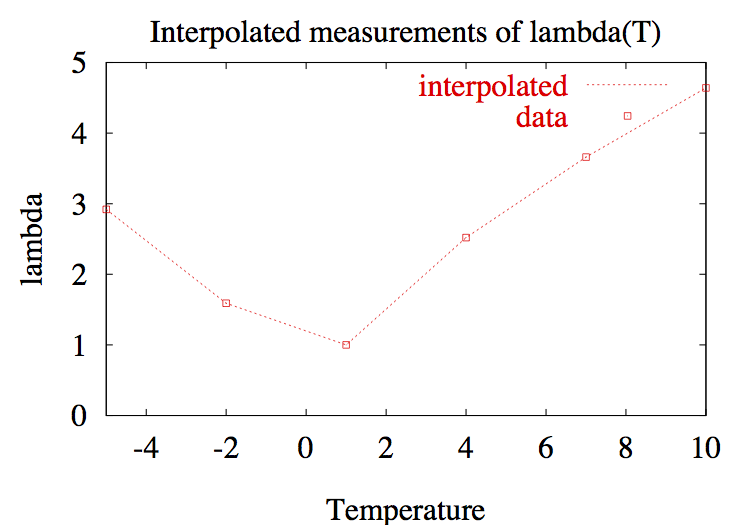
\includegraphics[height=3.5in]{table/table-interp.pdf}}
    \caption{A rock with $\lambda$ known only at a sequence of
      discrete temperature values, from experimental measurements.
      The function $\lambda(T)$  can be 
      represented approximately using linear interpolation (and the
      resulting approximate function can then be used to solve the
      problem numerically).}
    \label{lab1:fig:table}
  \end{figure}
\end{example}

As the above example demonstrates, even for a simple ODE such as
\eqref{lab1:eq:conduction1d}, there 
are situations where analytical methods are inadequate.  

%%%%%%%%%%%%%%%%%%%%%%%%%%%%%%%%%%%%%%%%%%%%%%%%%%%%%%%%%%%%%%%%%%%%%%%
\subsection{Partial Differential Equations}

\begin{example}
  \label{lab1:exm:diffusion1d}
  The rock in Example~\ref{lab1:exm:conduction} was considered to be small
  enough that the effects of heat diffusion in the interior
  were negligible in comparison to the heat lost by conduction
  through its surface.  
  In this example, consider a rock that is \emph{not small}, and whose
  temperature changes are dominated by internal diffusion effects.
  Therefore, it is no longer possible to ignore the spatial dependence
  in the problem.  

  For simplicity, we will add spatial dependence in one direction
  only, which corresponds to a ``one-dimensional rock'', or a thin
  rod.  Assume that the rod is insulated along its sides, so that heat
  flows only along its length, and possibly out the ends (see
  Figure~\ref{lab1:fig:rock-1d}).
  \begin{figure}[htbp]
    \begin{center}
      \leavevmode
%%%%%%%%%%%%%%%%%%%%%%%%%%%%%%%%%%%%%%%%%%%%%%%%%%%%%
%  NOTE: This plot is produced by the Gnuplot script
%  ``conduction/rod.gin''.
%%%%%%%%%%%%%%%%%%%%%%%%%%%%%%%%%%%%%%%%%%%%%%%%%%%%%
%      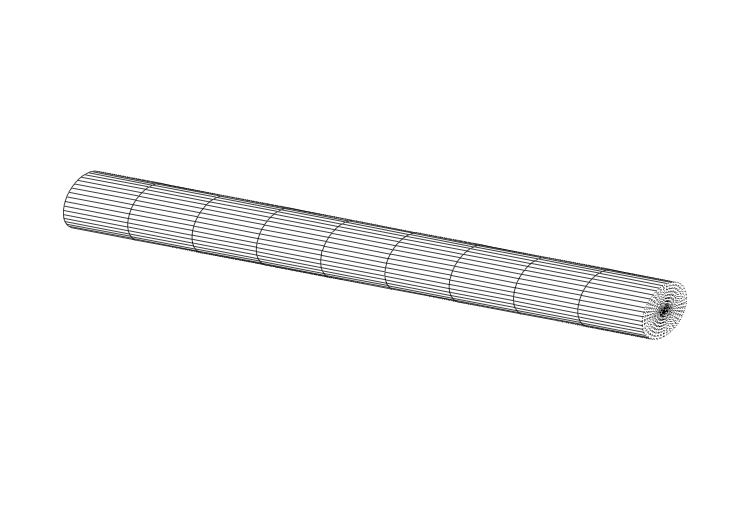
\includegraphics[width=4.5in]{conduction/rod.pdf}
      \caption{A thin rod can be thought of as a model for a
        one-dimensional rock.} 
      \label{lab1:fig:rock-1d}
    \end{center}
  \end{figure}
  Consequently, the temperature varies only with position, $x$, and
  time, $t$,
  and can be written as a function $u(x,t)$.   
  The temperature in the rod is governed by the following PDE
  \[
    u_t = \alpha^2 u_{xx},
  \]
  for which we have to provide an initial temperature 
  \[ 
    u(x,0) = u_0(x),
  \]
  and boundary values
  \[
    u(0,t)=u(1,t)=0,
  \]
  where 
  \begin{itemize}
  \item[$\circ$] $\alpha^2$ is the \emph{thermal diffusivity} of the
    material, 
  \item[$\circ$] $u_0(x)$ is the initial temperature distribution in the
    rod,  and
  \item[$\circ$] the boundary conditions indicate that the ends of the rod
    are held at constant temperature, which we've assumed is zero.
  \end{itemize}

  Thermal diffusivity is a quantity that depends only on the
  material from which the bar is made.  It is defined by 
  \[
  \alpha^2 = \frac{\kappa}{\rho c},
  \]
  where $\kappa$ is the thermal conductivity, $\rho$ is the density,
  and $c$ is the specific heat.  A typical value of the thermal
  diffusivity for a granite 
  bar is $0.011\;cm^2/sec$, and $0.0038\;cm^2/sec$ for a bar made of
  brick.  

  Using the method of \emph{separation of variables}, we can look for a
  temperature function of the form $u(x,t)=X(x) \cdot T(t)$, which leads to
  the infinite series solution
  \[
    u(x,t) = \sum_{n=1}^\infty b_n e^{-n^2\pi^2\alpha^2 t}\sin{(n\pi x)},
  \]
  where the series coefficients are
  \[
    b_n = 2 \int_0^1 u_0(x) \sin{(n\pi x)} dx.
  \]
%%%%%%%%%%%%%%%%%%%%%%%
\begin{latexonly}
  \gloss{separation of variables}{a technique whereby a function with
    several dependent variables is 
    written as a product of several functions, each of which depends
    on only one of the dependent variables.
    For example, a function of three unknowns, $u(x,y,t)$, might be
    written as $u(x,y,t)=X(x)\cdot Y(y) \cdot T(t)$.} 
\end{latexonly} 
%%%%%%%%%%%%%%%%%%%%%%%
  
  \begin{mathnote}
    Details of the derivation can be found in any introductory text in
    PDE's (for example, \cite[p.~549]{boyce-diprima}).  
  \end{mathnote}

  We do manage to obtain an explicit formula for the solution, which can
  be used to calculate actual values of the solution.  However, there
  are two obvious reasons why this formula is not of much
  practical use:
  \begin{enumerate}
  \item The series involves an infinite number of terms (except for
    very special forms for the initial heat distribution \dots\ such as
    the one shown below).  
    We might be able to truncate the series, since each term
    decreases exponentially in size, but it is not trivial to decide
    how many terms to choose in order to get an accurate answer and 
    here we are already entering the realm of numerical
    approximation.  
  \item Each term in the series requires the evaluation of an
    integral.  When these cannot be integrated analytically, we must
    find some way to approximate the integrals \dots\ numerical
    analysis rears its head once again!
  \end{enumerate}
  For most physical problems, an analytical expression cannot be
  obtained, and the exact formula is not of much use.  

  However, consider a very special case, when 
%% $\alpha^2$ is a constant, and
  the initial temperature distribution is sinusoidal, \ie
  \[
    u_0(x) = sin(\pi x).
  \]
  For this problem, the infinite series collapses into a single term
  \[
    u(x,t) = e^{-\pi^2\alpha^2t}\sin{\pi x}.
  \]

\begin{latexonly}
    Sample solution curves are given in Figure~\ref{lab1:fig:diffusion-1d}.
    \begin{figure}[htbp]
      \begin{center}
        \leavevmode
%%%%%%%%%%%%%%%%%%%%%%%%%%%%%%%%%%%%%%%%%%%%%%%%%%%%%
%  NOTE: This plot is produced by the Gnuplot script
%  ``diffusion/diffusion.gin''.
%%%%%%%%%%%%%%%%%%%%%%%%%%%%%%%%%%%%%%%%%%%%%%%%%%%%%
%        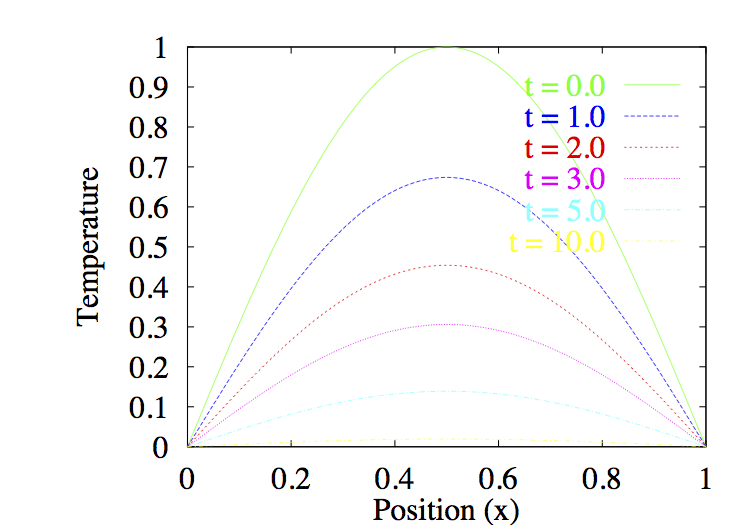
\includegraphics[height=3.5in]{diffusion/diffusion.pdf}
        \caption{Temperature vs.\ position curves at various times, for
          heat diffusion in a rod with sinusoidal initial
          temperature distribution and parameter value $\alpha=0.2$.} 
        \label{lab1:fig:diffusion-1d}
      \end{center}
    \end{figure}
\end{latexonly}

%%%%%%%%%%%%%%%%%%%%%%%%%%%%%%%%%%%%%%%%%%%%%%%%%%%%%
%  NOTE: This MPEG movie was generated first as a 
%  sequence of GIF images using the perl script
%  ``diffusion/genplots.pl'', which uses the package
%  pgperl.  
%  Then, the 31 GIF images were converted to an MPEG
%  movie by calling the ``makempeg script:
%
%     makempeg -fs 0 -fe 30 -fi 1 -base exact -ext gif
%
%%%%%%%%%%%%%%%%%%%%%%%%%%%%%%%%%%%%%%%%%%%%%%%%%%%%%
\movie{exact.mpg}{Here is a movie of the exact solution to the
  diffusion problem.}

Notes on viewing movies:  Once the window comes-up on your screen
move the cursor into the movie window, otherwise the colour palette
is incorrect.  If no movie window comes-up it is probably because
there is no mpeg viewer on your system.


%\demo{diffusion-1d.cgi}{To investigate the behaviour of the solution,
%  try out this interactive example -- NOT AVAILABLE YET!\label{lab1:demo:diffusion-1d}} 
%
%%%%%%%%%%%%
\begin{latexonly}
\gloss{linear}{pertaining to a function or expression in which the
  quantities appear in a linear combination.  If $x_i$ are the
  variable quantities, and $c_i$ are constants, then any linear
  function of the $x_i$ can be written in the form
  $c_0 + \sum_i c_i \cdot x_i$.}  
\gloss{non-linear}{pertaining to a function or expression in which the
  quantities appear in a non-linear combination.}
\gloss{Navier-Stokes equations}{the system of non-linear PDE's that
  describe the time evolution of the flow of a fluid.}
\end{latexonly}
%%%%%%%%%%%%
\end{example}

%%%
%%% \begin{example}
  Many flows in the atmosphere and ocean are governed by the
  Navier-Stokes equations, which are a complicated, non-linear system
  of PDE's, relating the evolution of pressure and velocity for a
  viscous fluid.
  Let us consider a simplified model of fluid motion, in
  which the flow is in the $x$-direction only, and pressure effects
  are ignored.  For this situation, the Navier-Stokes equations reduce
  to a single, non-linear partial differential equation in the
  velocity only:
  \[
    \underbrace{u_t}_{\mbox{time-dependence}} +
    \underbrace{uu_x}_{\mbox{advection}} 
    = \underbrace{\nu u_{xx}}_{\mbox{diffusion}}, 
  \]
  where $\nu$ is the {\em kinematic viscosity}.
  This equation is commonly known as {\em Burger's equation}. 

  \begin{mathnote}
    \hyperref{Details on the derivation from the Navier-Stokes
      equations \dots}{See Appendix }{ for an 
      an overview of the Navier-Stokes equations and the
      derivation of Burger's equation.}{lab1:ap:burgers} 
  \end{mathnote}

  In order that the problem have a unique solution, we must also
  impose the initial values
  \[
    u(x,0) = u_0(x).
  \]
  If we look for a solution without imposing any boundaries, and take
  $\nu$ to be constant, then the exact solution can be found as 
  \[
    u(x,t) = -2\nu \log \left[ \frac{1}{2 \sqrt{\pi \nu t}}
      \int_{-\infty}^\infty e^{-u_0(y)/2\nu} e^{-(x-y)^2/4\nu t}dy\right]. 
  \]
  If you thought that the solution to the heat equation problem in the
  previous example was impractical, then this solution is even worse!

  \begin{mathnote}
    \hyperref{Details of the derivation \dots}{See Appendix }{ for an  
      a derivation of the solution.}{lab1:ap:burgers-soln} 
  \end{mathnote}
\end{example}


%%%

\paragraph{Summary}

This section is best summed up by the insightful comment of
~\cite[p.~587]{strang-am}:  
\begin{quote}
  \centerline{\bf Nature is nonlinear.}
\end{quote}
Most problems arising in physics (which are non-linear) cannot be solved
analytically, or result in expressions that have little practical
value, and we must turn to numerical solution techniques.

%%% Local Variables: 
%%% mode: latex
%%% TeX-master: "lab1"
%%% End: 
